\documentclass[11pt, oneside]{article}   	% use "amsart" instead of "article" for AMSLaTeX format
\usepackage{geometry}                		% See geometry.pdf to learn the layout options. There are lots.
\geometry{letterpaper}                   		% ... or a4paper or a5paper or ... 
%\geometry{landscape}                		% Activate for for rotated page geometry
%\usepackage[parfill]{parskip}    		% Activate to begin paragraphs with an empty line rather than an indent
\usepackage{graphicx}				% Use pdf, png, jpg, or eps� with pdflatex; use eps in DVI mode
								% TeX will automatically convert eps --> pdf in pdflatex		
\usepackage{amssymb}
\usepackage{amsmath}
\usepackage{parskip}

\title{Torus:  parametrization and surface area}
%\author{The Author}
\date{}							% Activate to display a given date or no date
\graphicspath{{/Users/telliott_admin/Dropbox/Tex/png/}}

\begin{document}
\maketitle
%\section{}
%\subsection{}
\Large
The general theory which allows us to calculate surface areas includes a formula for parametrized surfaces.  

For parametrization of a line or a curve we need only one variable.
\[ x = \cos t \ \ \ \  y = \sin t \ \ \ \ z = ct \]
where $t$ is the parameter and $c$ is a constant, is the parametrization of a helix.

For a surface (like a sphere, or a torus), we will need two parameters, which are usually called $u$ and $v$. 
\begin{center} 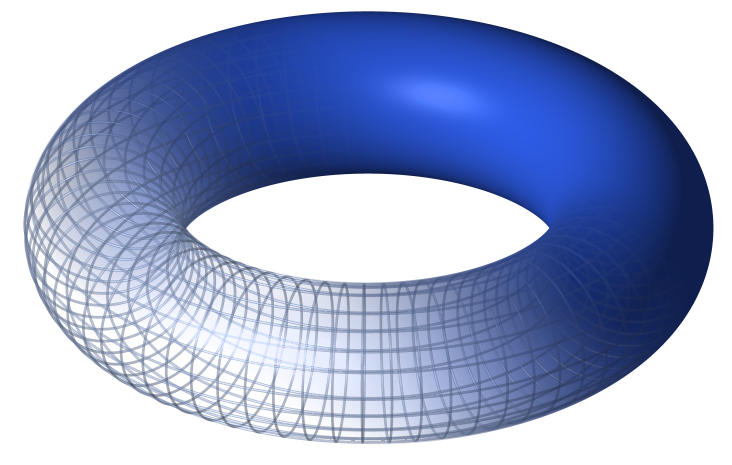
\includegraphics [scale=0.4] {torus.png} \end{center}
To get the surface area, we will just calculate 
\[ V = \int \ du \ dv \]
over the appropriate range of the two variables.  There is an additional constant:  we need to figure out the exchange rate for the surface area element $dS$  (composed of sides $du$ and $dv$) to units of $dA$ (composed of $dx$ and $dy$).  More about that later.

A torus is like a small circle moved around in a larger circle.  The small circle is the cross-section of the donut (radius $r$), while the large circle traces out the path of the donut (radius $R$).  Our parameters will be the angles $\theta$ and $\phi$.  $\theta$ describes the position of on the large circle (the position of the center of the small circle) as 
\[ x_c = R \cos \theta \ \ \ \  y_c = R \sin \theta \]
In this approach, the donut's axis of symmetry is the $z$-axis, and the body of the donut is centered half above the $xy$-plane and half below it.  The second angle, $\phi$, describes where we are on the small circle.  In particular, the distance above or below the $xy$-plane will be
\[ z = r \sin \phi \]
The only tricky part is the finaly adjustment to obtain the actual $x$ and $y$ coordinates.  For $x$, when $\phi = 0$, we go out from the origin an additional distance $r$, while when $\phi = \pi$, we subtract the same distance.  Our first attempt is:
\[ x = x_c + r \cos \phi \]
\[ = R \cos \theta + r \cos \phi \]
While this is correct for $\theta = 0$ it is not correct for other angles.  We need an additional factor of
$\cos \theta$:
\[ x = R \cos \theta + r \cos \phi \cos \theta \]
\[ = \cos \theta (R + r \cos \phi) \]
It may not be clear that this works for all angles, but if $\theta = \pi/2$ we add nothing additional to $x_c$, and that is just what we want.  Similarly for $y$
\[ y = y_c + r \cos \phi \sin \theta \]
\[ = \sin \theta (R  + r \cos \phi) \]

Now, according to the theory, what we need to do is take the partial derivatives of these functions with respect to $\theta$ and $\phi$.  For example:
\[ x_{\theta} = \frac{dx}{d \theta} = \frac{d}{d \theta} \ \cos \theta (R + r \cos \phi) \]
We find that
\[ x = \cos \theta (R + r \cos \phi) \]
\[ x_{\theta} = -\sin \theta (R + r \cos \phi) \]
\[ x_{\phi} = -\cos \theta \ r \sin \phi \]
while
\[ y = \sin \theta (R  + r \cos \phi) \]
\[ y_{\theta} = \cos \theta (R + r \cos \phi) \]
\[ y_{\phi} = -\sin \theta \ r \sin \phi \]
$z$ does not depend on $\theta$ so
\[ z_{\theta} = 0 \]
\[ z_{\phi} = r \cos \phi \]
The position vector to a point on the surface is
\[ \mathbf{r} = \ \langle x,y,z \rangle \]
\[ \mathbf{r_{\theta}} = \ \langle x_{\theta},y_{\theta},z_{\theta} \rangle \]
\[ \mathbf{r_{\phi}} = \ \langle x_{\phi},y_{\phi},z_{\phi} \rangle \]

The unit for conversion is called the Jacobian.  It is the length of the vector $\mathbf{r_{\theta}} \times \mathbf{r_{\phi}}$.  It's a bit complicated, so let's do the pieces individually.  The vector product has three terms
\[ \hat{\mathbf{i}} \ y_{\theta} z_{\phi} -  y_{\phi} z_{\theta} \]
\[ = \hat{\mathbf{i}} \  \cos \theta (R + r \cos \phi) r \cos \phi - 0 \]
\[ \hat{\mathbf{j}} \ x_{\phi} z_{\theta} -  x_{\theta} z_{\phi} \]
\[ = \hat{\mathbf{j}} \  0 - \sin \theta (R + r \cos \phi) r \cos \phi  \]
The third term is most complicated
\[ \hat{\mathbf{k}} \ x_{\theta} y_{\phi} -  x_{\phi} y_{\theta} \]
\[ = \hat{\mathbf{k}} \sin \theta (R + r \cos \phi) \sin \theta \ r \sin \phi + \cos \theta \ r \sin \phi \cos \theta (R + r \cos \phi) \]
But notice that we have the same term times $\sin^2 \theta$ and $\cos^2 \theta$ so this reduces immediately to 
\[ = \hat{\mathbf{k}}  (R + r \cos \phi) \ r \sin \phi \]

The next (and nearly the last) step is to calculate the length of this vector, by squaring each term and adding.  Before we do that, notice that all three components contain a factor of $r (R + r \cos \phi)$.  We will leave that aside and remember it at the end.  The rest of the sum of squares is:
\[ \cos^2 \theta \cos^2 \phi + \sin^2 \theta \cos^2 \phi + \sin^2 \phi   \]
\[ = \cos^2 \phi + \sin^2 \phi  = 1 \]
So the factor we held aside is all that's left
\[ |\mathbf{r_{\theta}} \times \mathbf{r_{\phi}} | = r (R + r \cos \phi) \]

And the surface integral is just
\[ A_S = \int dS = \int_{\theta = 0}^{2 \pi} \int_{\phi = 0}^{2 \pi} |\mathbf{r_{\theta}} \times \mathbf{r_{\phi}}| \ d \phi \ d \theta \]
\[ = \int_{\theta = 0}^{2 \pi} \int_{\phi = 0}^{2 \pi} r (R + r \cos \phi) \ d \phi \ d \theta \]

Since $\theta$ is independent of $\phi$ and $R$ and $r$, we get
\[ = 2 \pi r  \int_{\phi = 0}^{2 \pi} (R + r \cos \phi) \ d \phi  \]
But the integral of $\cos \phi$ is just $\sin \phi$, which is zero at the upper and lower bounds on $\phi$, hence 
\[ = 2 \pi r  \int_{\phi = 0}^{2 \pi} R \ d \phi  \]
\[ = 2 \pi r  \ 2 \pi R \]
Which is pretty amazing.  We go around the torus along what is called its centroid, traveling a distance $ 2 \pi R$.  At each point we have the circumference of the small circle, which is $ 2 \pi r$.  

It seems strange that the curvature doesn't make any difference.  There is a theorem in geometry (the Theorem of Pappus), with the same result.  

Pappus also allows us to calculate the volume as
\[ V = \pi r^2 \ 2 \pi R \]

\end{document}  